\begin{minipage}[t]{180mm}
\fcolorbox{black}{white}{
\begin{minipage}[b]{30mm}

\includegraphics[width=0.5\linewidth]{unflogo.pdf}
\end{minipage}
\begin{minipage}[b]{100mm}
\Huge \textbf{UNF NEWZ} \\
\Large -- Søvn og retsstavning er overvurderet! 
\end{minipage}
\begin{minipage}[b]{50mm}
\Large Onsdag 17.07.2015 \\
\normalsize Redigeret i \LaTeX\ af \\ SOM, MGS, MMN, SABH
\end{minipage}
}
\end{minipage}



\begin{minipage}[b]{0.95\linewidth}
\begin{minipage}[t]{0.47\textwidth}
\vspace{3mm}
\section*{Dagens mediciner}


\section*{Ordforklaring: }

\end{minipage}%
\hfill\begin{minipage}[t]{0.47\textwidth}
\vspace{3mm}
\section*{Vejrudsigt}
\textbf{IMF, AU (fra DMI)}: 

\textbf{X}: 

\section*{Find en Fynbo}

\section*{Fakt om Jylland}
Ifølge den jyske metrik er alt under $25$ km gåafstand.

\section*{Dagens sandsynlighed}

\vspace{3mm}
\end{minipage}

%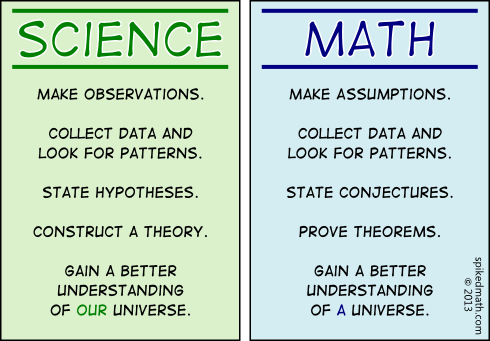
\includegraphics[width=\textwidth]{542-science-vs-math.png}
\begin{center}
\tiny Mike, http://spikedmath.com/542.html, CC-BY-NC-2.5

\vspace{3mm}

\tiny UNF Newz er avisen hvor at ansvarshavende redaktør fralægger sig ethvert ansvar for eventuel plagiering, kaniner, tysk, stavefelj, kaffe, dårlig humor, glemsomhed, katte, store sigmaer, pile, skyer, dårlige oversættelser og alt hvad eventuelle homo sapiens sapiens kunne finde på at holde imod UNF Newz! Dog tager UNF Newz fuld credit og copyright for alle guldkorn, magickort, mus, \TeX, humor, smil, Mortener, kaffe, før-fremtid, ringe og/eller rubik's cube.
\end{center}
\end{minipage}

